 \documentclass[11pt, oneside]{article} 
\usepackage{geometry}
\geometry{letterpaper} 
\usepackage{graphicx}
	
\usepackage{amssymb}
\usepackage{amsmath}
\usepackage{parskip}
\usepackage{color}
\usepackage{hyperref}

\graphicspath{{/Users/telliott_admin/Tex/png/}}
% \begin{center} 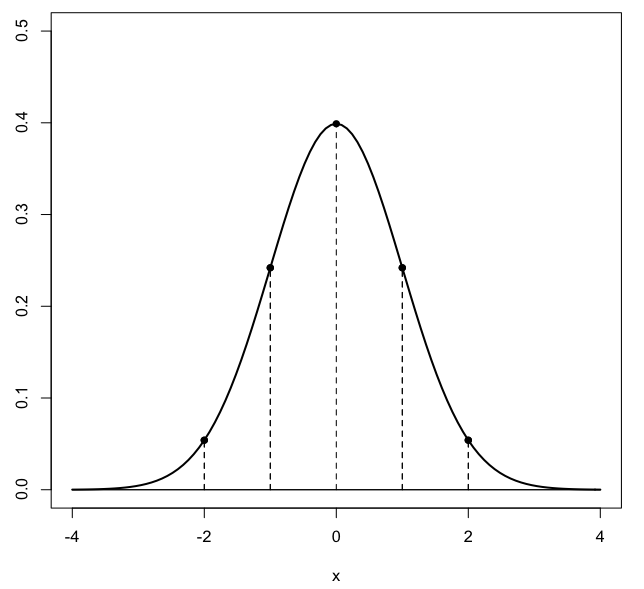
\includegraphics [scale=0.4] {gauss3.png} \end{center}

\title{Subsequences}
\date{}

\begin{document}
\maketitle
\Large

\section{Subsequences}

A subsequence of a sequence ($a_n$) is a sequence (an infinite collection of numbers) derived from ($a_n$) with elements in the same order that they appear in that sequence.  There is no requirement for how the elements are chosen.

The main theorem on subsequences is that every subsequence of a convergent sequence ($a_n$) converges to the same limit as ($a_n$).

However, knowing that a sequence ($a_n$)  has a single convergent subsequence says nothing about the convergence of ($a_n$) .

\subsection*{examples}

The only rule is that we must select an infinite number of terms and preserve the order.
\[ a_n = \frac{1}{1}, \frac{1}{2}, \frac{1}{3}, \frac{1}{4}, \dots = \frac{1}{n} \]
\[ \ \ b_n = \frac{1}{1}, \frac{1}{2}, \frac{1}{4}, \frac{1}{8}, \dots = \frac{1}{2^n} \]
$b_n$ is a subsequence of $a_n$.

The theorem says that 
\[ \lim a_n = \lim b_n \] 
and indeed, if we guess that the limit is zero we can satisfy the $\epsilon, \delta$ formalism.

\subsection*{a bounded sequence that does not converge}

Consider the sequence 
\[ a_n = (-1)^n  = -1, 1, -1, 1, \dots \]
Let $b_n$ consist of the odd numbered terms $b_n = -1, -1 \dots$ and $c_n = 1,1, \dots$.  Clearly these two limits are different.  We claim that $(a_n)$ does not converge.

\subsection*{proof}

Suppose that $a_n$ converges to some limit $L$.  The theorem says that the limits for $b_n$ and $c_n$ should both be equal to $L$, but they are different.  This is a contradiction.  Therefore $a_n$ does not converge.

\subsection*{Using subsequences to prove convergence}

The idea of "covering a sequence by subsequences" is to split all the terms of a sequence ($a_n$) into two subsequences and prove these two subsequences tend to the same limit. Often a sequence is split into its odd-numbered and its even-numbered terms. But it is essential to consider all the terms of the original sequence and ensure both subsequences tend to the same limit. Just knowing a sequence ($a_n$) has a convergent subsequence says nothing about the convergence of the whole sequence($a_n$).

\section{Cauchy Sequences}

We've established that knowing that a sequence has a limit (and what that limit is) allows us to show that it converges.  But we'd like to establish that a sequence is convergent without knowing the limit.

The idea of "Cauchy sequences" is that in a convergent sequence, as the terms get closer and closer to the limit, they are also getting closer and closer to each other.

A sequence $(a_n)$ is called \textbf{Cauchy} if and only if

\[ \forall \ \epsilon > 0, \exists \ N \in \mathbb{N} \ | \ m, n > N \Rightarrow |a_n - a_m| < \epsilon \]

The Cauchy criterion is that not only do adjacent terms become closer and closer together, but after a certain point, \emph{all} terms of the sequence become close together.

We note that the inequality $| x_m  - x_n | < \epsilon$ must be valid for all integers $m,n > N$.  In particular, a sequence $(x_n)$ satisfying only $|x_{n+1} -  x_n | < \epsilon$ for all $n > N$ may not be a Cauchy sequence.

\subsection*{example}
??

\subsection*{results about Cauchy sequences}

$\bullet$  Every Cauchy sequence is bounded.

$\bullet$  A sequence of real numbers converges if and only if it is a Cauchy sequence.

\subsection*{theorem}

A sequence of real numbers converges if and only if it is a Cauchy sequence.

\subsection*{forward proof} 
??

\subsection*{reverse proof} 

Suppose that $(a_n)$ is convergent and the limit of $(a_n)$ is $L$.  

Let $\epsilon > 0$ and let $N \in \mathbb{N}$ be such that $n > N \Rightarrow$ $| a_n - L | < \epsilon / 2$.

Then $m > n > N$ implies that both $|a_n - L| < \epsilon / 2$ and $|a_m - L| < \epsilon / 2$.

\[ |a_n - a_m| = |(a_n - L) - (a_m - L)| \]
By the triangle inequality
\[ |(a_n - L) - (a_m - L)| \le | a_m - L | + | a_n - L | \]
\[ | a_m - L | + | a_n - L | = \epsilon \]
so
\[ |a_n - a_m| <  \epsilon \]
Therefore $(a_n)$ satisfies the Cauchy criterion.

\subsection*{theorem:  Bolzano-Weierstrass}

\url{theoremoftheweek.wordpress.com/2010/03/10/theorem-20-the-bolzano-weierstrass-theorem/}

$\bullet$  Every bounded sequence has a convergent subsequence.

Suppose the sequence $(a_n)$ is bounded and lies (say) in the interval $[0,1]$.  We construct a convergent sequence by a bisection process.  

Split the interval $I = [0,1]$ into two halves:  $[0,1/2]$ and $[1/2,1]$.  Then (at least) one of the intervals will have infinitely many terms.  Suppose the interval $I_1' = I[0,1/2]$ has infinitely many terms.  We focus on it now.

Among the terms in $I_1'$, choose the term that appears first in the original sequence $(a_n)$  Call it $x_1$.

Then, split $I_1'$ in half to give $I_2'$ and $I_2''$.  Repeat the process, choose one of the intervals with the provision that it has an infinite number of terms, and letting $x_2$ be the first term from the original series that lies in that interval.

Note that $x_2$ must come later in the series $(a_n)$ than $x_1$ does. 

Continuing in this way, we form $(x_n)$, which is a subsequence of $(a_n)$.  

$(x_n)$ lies in an interval $[a_n,b_n]$.

Furthermore, the bounds of the intervals have the property that
\[ a_1 \le a_i \le a_{i+1} \le b_{i+1} \le b_i \le b_1 \]

\subsection*{claim}

The subsequence $(x_n)$ is convergent.

\subsection*{proof}
The sequence of "left-hand ends" of intervals is monotonic increasing, bounded above by $1$, hence with limit $\alpha$.  The sequence of right-hand ends is monotonic decreasing, bounded below by $0$, with limit $\beta$.

Let $\epsilon > 0$.  We can choose $n$ so that all the terms of the sequence $a_m, m > n$ lie within $\pm \epsilon$ of the center of the interval $I_n$.

Since the length of the interval shrinks like $(1/2)^n$, converging to $0$, we must have $\beta - \alpha = 0$, thus $\alpha = \beta$.

Since the infinite sequence is trapped between the sequence of left-hand and right-hand ends, by the squeeze theorem, it converges to the same limit.

\subsection*{restate the theorem}

$\bullet$  Every bounded sequence has a convergent subsequence.

\subsection*{proof 2}
Consider a bounded sequence $(a_n)$ of real numbers.  We will show that it has a monotone subsequence.  Since it's montonic and bounded, this subsequence then converges to a limit.

Let's say that a value $a_n$ in the sequence is a peak or summit if $a_n \ge a_m$ for all $m > n$.  

We make a list of the peaks:  call them $x_1, x_2, \dots$.  

The list is monotone decreasing $x_1 \ge x_2$, etc.  But the dots are slightly misleading, since the subsequence may be finite.

\subsection*{infinite}

If there are infinitely many peaks, then there is an infinite monotone decreasing subsequence $(x_1, x_2 \dots)$. 

\subsection*{finite}

There is a finite number of peaks.  Find the last one.  

This is an element with no larger elements coming later in the (infinite) sequence, and each subsequent element has the same property.  The sequence from this point must be monotone increasing.

$\square$






\end{document}